\section{Wheeler and $p$-sortable Graphs}
\label{sec:wheeler_and_psortable_graphs}

\subsection{Introduction and Motivation}
As established in the introduction, the primary goal of this thesis is to find an effective balance between compressing a finite language and preserving its indexability. The two extremes—full DFA minimization and the raw input trie—are inadequate, as one sacrifices indexing for compression and the other sacrifices compression for indexing. The solution to this problem lies in a specific class of graphs that are structured enough to be indexed efficiently yet flexible enough to allow for significant compression. This chapter introduces the theoretical framework that underpins our approach: Wheeler graphs and their generalization, $p$-sortable graphs.

A crucial observation is that the input trie representing our language is already a highly structured object. It is a Wheeler graph, a type of graph that admits a special ordering on its nodes and edges, making it exceptionally well-suited for indexing. In formal terms, a trie is a 1-sortable graph. This property explains both its powerful indexing capabilities and its inherent lack of compression.

The concept of $p$-sortability offers a way to navigate the trade-off. By controllably increasing the sortability parameter $p$, we can begin to merge MN-equivalent states (see \cref{def:myhill-nerode}), thereby compressing the graph. The resulting automaton is no longer a simple trie but a more general $p$-sortable graph that retains strong indexing properties. This chapter will formally define these concepts, which are the foundation of our algorithm for achieving a practical compromise between compression and indexability.

\subsection{Orders}
The core property that makes Wheeler and $p$-sortable graphs efficiently indexable is the existence of a specific ordering on their states. This ordering provides the necessary structure to navigate the automaton and answer queries quickly, a task that is computationally hard on general graphs. The fundamental ordering used in this context is the \textit{co-lexicographic order} (co-lex), which compares states based on the labels of the paths that reach them. This section formally defines this order and the related concepts that are essential for understanding the structure of indexable automata.

\begin{definition} [Co-lexicographic Order on $\Sigma^*$]
    The co-lex order $\preceq$ is defined as follows. Given two strings $\alpha, \beta \in \Sigma^*$, we say that $\alpha \preceq \beta$ if and only if either:
    \begin{itemize}[leftmargin=25pt]
        \item $\alpha$ is a suffix of $\beta$, or
        \item there exist strings $\alpha', \beta', \gamma \in \Sigma^*$ and symbols $a, b \in \Sigma$, such that $\alpha = \alpha'a\gamma$, $\beta = \beta'b\gamma$, and $a \prec b$.
    \end{itemize}
\end{definition}

Now, let's define the formal concept of partial order and the width of a partial order. 
\begin{definition}[Partial Order]
    A partial order is a binary relation $\leq$ over a set $S$ that is reflexive, antisymmetric, and transitive. That is, for all $a, b, c \in S$:
    \begin{itemize}[leftmargin=25pt]
        \item $a \leq a$ (reflexivity)
        \item if $a \leq b$ and $b \leq a$, then $a = b$ (antisymmetry)
        \item if $a \leq b$ and $b \leq c$, then $a \leq c$ (transitivity)
    \end{itemize}
\end{definition}

A partial order $(S, \leq)$ can be visualized using a \textit{Hasse diagram}. In a Hasse diagram, each element of $S$ is represented by a node, and given $a,b,c \in S$ there is a line segment or curve going upward from $a$ to $b$ if $a \leq b$ and there is no element $c$ such that $a \leq c \leq b$. The direction of the relation is implicitly understood to be upwards, so arrows are not needed. Also, if two elements of $S$ are incomparable under $\leq$ they are displayed at the same level in the diagram. An example is given in \cref{ex:hasse}.

\begin{example} \label{ex:hasse}
    In the example shown in \cref{fig:hasse_diagram_example}, the set is composed of the divisors of 12, and the relation is divisibility. An edge is drawn from $a$ to $b$ if $a$ divides $b$ and there is no other element $c$ in the set such that $a/c$ and $c/b$. For instance, there is an edge from 2 to 4 because 2 divides 4, and no other element in the set is a multiple of 2 and a divisor of 4. There is no direct edge from 2 to 12 because the relationship is captured transitively through other elements, such as $2/4/12$ or $2/6/12$.
    \begin{figure}[H]
        \centering
        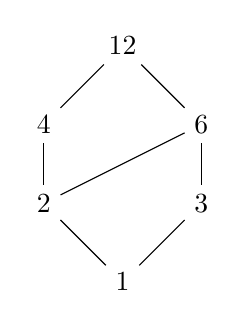
\begin{tikzpicture}[node distance=1.5cm]
            \node (1) at (0,0) {1};
            \node (2) at (-1,1) {2};
            \node (3) at (1,1) {3};
            \node (4) at (-1,2) {4};
            \node (6) at (1,2) {6};
            \node (12) at (0,3) {12};

            \draw (1) -- (2);
            \draw (1) -- (3);
            \draw (2) -- (4);
            \draw (2) -- (6);
            \draw (3) -- (6);
            \draw (4) -- (12);
            \draw (6) -- (12);
        \end{tikzpicture}
        \caption{Hasse diagram for the set $\{1, 2, 3, 4, 6, 12\}$ with the "divides" relation.}
        \label{fig:hasse_diagram_example}
    \end{figure}
\end{example}

Now we can define the concept of width of a partial order.

\begin{definition}[Antichain]
    An antichain of a partially ordered set $(S, \leq)$ is a subset of $S$ where any two distinct elements are incomparable. That is, for any two distinct elements $a, b$ in the antichain, neither $a \leq b$ nor $b \leq a$ holds.
\end{definition}

\begin{definition}[Width of a partial order, \cite{dilworth1990decomposition}]
    The width of a partially ordered set is the size of the largest possible antichain.
\end{definition}

By Dilworth's Theorem \cite{dilworth1990decomposition}, the width of a partially ordered set $(S, \leq)$ is equal to the cardinality of its largest antichain; this can be equivalently defined as the minimum number of chains needed to partition $S$, where each chain is a totally ordered subset of $S$ under the relation $\leq$. 

\subsection{Wheeler Graphs}
With the concept of co-lex order established, we can now define the class of graphs that form the starting point of our work. A Wheeler automaton is an automaton where the states can be arranged in a strict, total order.

\begin{definition}[Wheeler automaton, \cite{gagie2017wheeler}]
    \label{def:wheeler_automaton}
    A finite state automaton \\
    $\mathcal{A} = (Q, \Sigma, \delta, q_0, F)$ is a \textit{Wheeler automaton} if there exists a total order $\leq$ on its set of states $Q$ that satisfies the following axioms:
    \begin{enumerate}[leftmargin=25pt]
        \item The initial state precede all other states in the order.
    \suspend{enumerate}
    For any two transitions $u \in \delta(u', a)$ and $v \in \delta(v', b)$:
    \resume{enumerate}[{[leftmargin=25pt]}]
        \item $a<b \implies u \leq v$,
        \item $a=b \wedge u' < v' \implies u \leq v$.
    \end{enumerate}
    The order $\leq$ is called a \textit{Wheeler order}.
\end{definition}

Consequently, we define the concept of Wheeler language.
\begin{definition}[Wheeler language]
    A Wheeler language $L$ is a language accepted by a deterministic Wheeler automaton.
\end{definition}

The most important example for Wheeler automaton in this thesis is the trie. Any trie representing a finite language is a Wheeler automaton. The co-lexicographic order of the strings spelling the paths from the root to each node provides the required total ordering of the states. This is why tries are inherently indexable. However, this rigid structure also means they are uncompressed, as every unique path must be stored explicitly, even if it corresponds to a substring that appears many times in the language. Our work begins with this observation: we start with a Wheeler automaton (the trie) and seek to compress it while preserving efficient indexability.

\subsection{The Co-lex Width of an Automaton}
Now that we have the concepts of co-lex order and width, we can combine them to formally define the class of indexable automata that are central to this thesis. The width of the co-lex partial order on an automaton's states is the critical measure of its structural complexity from an indexing perspective.

The co-lex order can be extended to the set of states of an automaton. The idea of co-lex order on the states of an automaton was first introduced with the notion of Wheeler graphs by Gagie et al.~\cite{gagie2017wheeler} and was later generalized to arbitrary finite automata by Cotumaccio and Prezza~\cite{cotumaccio2021indexing}, where a partial order replaces the total order. The definition of co-lex order on an automaton is as follows:

\begin{definition}[\cite{cotumaccio2023co}]
    \label{def:colex_order_on_automaton}
    Let $N = (Q, \Sigma, \delta, q_0, F)$ be an NFA. A co-lex order on $N$ is a partial order $\leq$ on $Q$ that satisfies the following two axioms:
    \begin{enumerate}[leftmargin=25pt]
        \item For every $u, v \in Q$, if $u < v$, then $\max\lambda(u) < \min\lambda(v)$
        \item For every $a \in \Sigma$ and $u, v, u', v' \in Q$, if $u \in \delta(u', a)$, $v \in \delta(v', a)$ and $u < v$, then $u' \leq v'$
    \end{enumerate}
\end{definition}
Where $\lambda(q)$ denotes the set of labels of transitions entering state $q$, and $\min\lambda(q)$ and $\max\lambda(q)$ represent the minimum and maximum element of the set, respectively.

The two axioms in \cref{def:colex_order_on_automaton} allow for pair of states of a finite automaton to be compared. When $\leq$ is total, we say that the co-lex order is a Wheeler order (introduced in \cite{gagie2017wheeler}). 

Consequently, we can introduce the concept of co-lex width of an automaton.
\begin{definition}[\cite{cotumaccio2023co}]
    The co-lex width of an NFA N is the minimum width of a co-lex order on N.
    $$
        width(N) = \min \{width(\leq)|\leq \text{ is a co-lex order on } N\}
    $$
\end{definition}

The requirement of a Wheeler order is powerful but restrictive. Many automata, especially those resulting from DAG compression, may not satisfy it (see \cref{ex:incomparability}). This introduces a fundamental trade-off: while DAG compression minimizes an automaton's size, it can destroy the very structure that enables efficient indexing. In fact, it has been shown that indexing general graphs—and thus, highly compressed automata—to support fast string matching is computationally expensive, as showed in \cite{equiGraphsCannotBe2023}. The second axiom of \cref{def:colex_order_on_automaton} does not always enforce an ordering between any two states, leading to a partial order instead of a total one. This gives rise to the more general notion of a \textit{$p$-sortable automaton}, where $p$ is the co-lex width of the automaton (see \cref{ex:p-sortable}). Under this definitions, a Wheeler automaton is a \textbf{1-sortable automaton}, as a total order has a width of 1 (the largest antichain is a single element).

\begin{example} \label{ex:incomparability}
    State incomparability can arise in several situations. For example, consider two states $u$ and $u'$.
    \begin{itemize}
        \item As illustrated in Figure~\ref{fig:incomparability-scenarios-combined}-(a), if we have two same-labeled transitions where the target states $u$ and $v$ are incomparable, we have no information about the relative order of the source states $u'$ and $v'$. Consequently, they may also be incomparable.
        \item Conflicting constraints from different labels can force incomparability, as shown in Figure~\ref{fig:incomparability-scenarios-combined}-(b). An existing order on the sources of $a$-transitions (e.g., $u' < v'$) may require $u < v$ to satisfy the Wheeler axioms, while an order on the sources of $b$-transitions (e.g., $v'' < u''$) may require the opposite, $v < u$. Since both cannot be true, the targets $u$ and $v$ must be incomparable.
    \end{itemize}

    \begin{figure}[H]
    \centering
    \begin{subfigure}[b]{0.4\textwidth}
        \centering
        \begin{tikzpicture}[
            node distance=2.5cm, 
            on grid, 
            auto,
            state/.style={circle, draw, minimum size=1cm}
        ]
        % Scenario 1
        \node[state, initial, initial text=] (u') at (0,0) {$u'$};
        \node[state, accepting] (u) at (2.5,0) {$u$};
        \node[state, initial, initial text=] (v') at (0,-2.5) {$v'$};
        \node[state, accepting] (v) at (2.5,-2.5) {$v$};

        \path[->] (u') edge node {$a$} (u);
        \path[->] (v') edge node {$a$} (v);

        \node at (0, -3.5) {$u' \parallel v'$};
        \node at (2.5, -3.5) {$u \parallel v$};
        \end{tikzpicture}
        \caption{}
        \label{fig:incomparability-scenario1}
    \end{subfigure}
    \hfill
    \begin{subfigure}[b]{0.55\textwidth}
        \centering
        \begin{tikzpicture}[
            node distance=2.5cm, 
            on grid, 
            auto,
            state/.style={circle, draw, minimum size=1cm}
        ]
        % Scenario 2
        \node[state, initial, initial text=] (u'2) at (0,0) {$u'$};
        \node[state, accepting] (u2) at (2.5,0) {$u$};
        \node[state, initial, initial text=, initial where=right] (u''2) at (5,0) {$u''$};
        
        \node[state, initial, initial text=] (v'2) at (0,-2.5) {$v'$};
        \node[state, accepting] (v2) at (2.5,-2.5) {$v$};
        \node[state, initial, initial text=, initial where=right] (v''2) at (5,-2.5) {$v''$};
    
        \path[->] (u'2) edge node {$a$} (u2);
        \path[->] (u''2) edge node[above] {$b$} (u2);
        \path[->] (v'2) edge node {$a$} (v2);
        \path[->] (v''2) edge node[below] {$b$} (v2);

        \node at (0, -3.5) {$u' < v'$};
        \node at (2.5, -3.5) {$u \parallel v$};
        \node at (5, -3.5) {$v'' < u''$};
        \end{tikzpicture}
        \caption{}
        \label{fig:incomparability-scenario2}
    \end{subfigure}
    \caption{Examples of state incomparability in automata.}
    \label{fig:incomparability-scenarios-combined}
    \end{figure}
\end{example}

\begin{example} \label{ex:p-sortable}
    Consider the following DFA $D$ of \cref{fig:non_wheeler_example}-(a) and its partial co-lex order \cref{fig:non_wheeler_example}-(b). The DFA is not Wheeler because states $v_3$ and $v_5$ and states $v_4$ and $v_7$ are incomparable (as shown in the Hasse diagram). $D$ admits a partition into $2$ $\leq$-chains, for example one possible $\leq$-chain partition is given by:
    \begin{itemize}
        \item Chain 1: $v_1 \leq v_2 \leq v_3 \leq v_4$
        \item Chain 2: $v_5 \leq v_6 \leq v_7$
    \end{itemize}

    \begin{figure}[H]
        \centering
        \begin{subfigure}[b]{0.6\textwidth}
            \centering
            \begin{tikzpicture}[->, >=stealth, node distance=1.5cm, auto]
                \tikzset{
                    state/.style={circle, draw, minimum size=0.8cm},
                    accepting/.style={state, double}
                }

                \node[state, initial, initial text=] (v1) at (0,1) {$v_1$};
                \node[state] (v2) at (2,1) {$v_2$};
                \node[state] (v3) at (4,1) {$v_3$};
                \node[accepting] (v5) at (4,-1) {$v_5$};
                \node[accepting] (v6) at (6,1) {$v_6$};
                \node[state] (v7) at (8,1) {$v_7$};
                \node[accepting] (v4) at (8,-1) {$v_4$};

                \path (v1) edge node {a} (v2)
                      (v2) edge [bend left=30] node[above] {b} (v6)
                      (v6) edge [bend left=0] node[above] {a} (v3)
                      (v3) edge [bend left=20] node[right] {a} (v5)
                      (v5) edge [bend left=20] node[left] {a} (v3)
                      (v5) edge node[below] {b} (v7)
                      (v6) edge [bend right=0] node[above] {b} (v7)
                      (v7) edge [bend left=20] node[right] {b,c} (v4)
                      (v4) edge [bend left=20] node[left] {b} (v7);
            \end{tikzpicture}
            \caption{}
            \label{fig:non_wheeler_graph_example}
        \end{subfigure}%
        \hfill
        \begin{subfigure}[b]{0.35\textwidth}
            \centering
            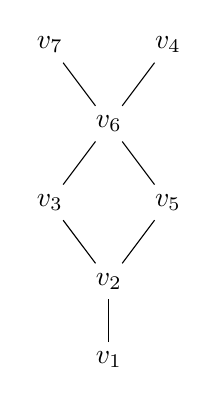
\begin{tikzpicture}
                \node (v1) at (0,0) {$v_1$};
                \node (v2) at (0,1) {$v_2$};
                \node (v3) at (-0.75,2) {$v_3$};
                \node (v5) at (0.75,2) {$v_5$};
                \node (v6) at (0,3) {$v_6$};
                \node (v4) at (0.75,4) {$v_4$};
                \node (v7) at (-0.75,4) {$v_7$};

                \draw (v1) -- (v2);
                \draw (v2) -- (v3);
                \draw (v2) -- (v5);
                \draw (v3) -- (v6);
                \draw (v5) -- (v6);
                \draw (v6) -- (v4);
                \draw (v6) -- (v7);
            \end{tikzpicture}
            \caption{}
            \label{fig:non_wheeler_graph_poset}
        \end{subfigure}
        \caption{An example of a $2$-sortable DFA and its corresponding Hasse diagram of the partial order.}
        \label{fig:non_wheeler_example}
    \end{figure}
\end{example}

We now introduce another important result by \cite{manziniRationalConstructionWheeler2024}. Let $D = (Q, \Sigma, \delta, s, F)$ denote the minimal DFA accepting a Wheeler language $L$, and let $D^w = (Q^w, \Sigma, \delta^w, s^w, F^w)$ denote the minimal Wheeler DFA (WDFA) accepting $L$. Since $D^w$ is Wheeler, the rational embedding ensures that for any two distinct states $q, q' \in Q^w$, the associated intervals $I_q, I_{q'}$ are disjoint. This property does not generally hold for $D$, where states may correspond to overlapping sets of prefixes. As a consequence, when transforming $D$ into $D^w$, certain states of $D$ may need to be \emph{split} into several states in $D^w$, potentially leading to an exponential blow-up in the number of states.

\begin{example}[\cite{manziniRationalConstructionWheeler2024}]
    We now provide a simple example of an automaton $D$ with width $n$ that accepts a Wheeler language, yet its minimum equivalent Wheeler DFA, $D^w$, is exponentially larger. Let $D$ be the automaton depicted in Figure~\ref{fig:exponential-gap-dfa}.

    \begin{figure}[H]
    \centering
    \begin{tikzpicture}[
        node distance=1.5cm and 2cm,
        auto,
        state/.style={circle, draw, minimum size=0.8cm, inner sep=0pt}
    ]
        \node[state, initial, initial text=] (start) at (0,0) {\#};
        
        \node[state] (w1_1) at (1.5,1.3) {1};
        \node[state] (w1_2) at (1.5,-1.3) {2};
        \node[state] (q1) at (3,0) {3};
        \node at (3, -0.7) {$q_1$};

        \path[->] (start) edge (w1_1);
        \path[->] (start) edge (w1_2);
        \path[->] (w1_1) edge node[above] {} (q1);
        \path[->] (w1_2) edge node[below] {} (q1);

        \node[state] (w2_1) at (4.5,1.3) {1};
        \node[state] (w2_2) at (4.5,-1.3) {2};
        \node[state] (q2) at (6,0) {3};
        \node at (6, -0.7) {$q_2$};
        \node at (4.5, -2) {$s_1$};
        \node at (4.5, 2) {$w_2$};

        \path[->] (q1) edge (w2_1);
        \path[->] (q1) edge (w2_2);
        \path[->] (w2_1) edge node[above] {} (q2);
        \path[->] (w2_2) edge node[below] {} (q2);

        \node at (7.5, 0) {$\cdots\cdots\cdots$};

        \node[state] (qn) at (9,0) {3};

        \node[state] (wn_1) at (10.5,1.3) {1};
        \node[state] (wn_2) at (10.5,-1.3) {2};
        \node[state, accepting] (t) at (12,0) {3};
        \node at (9, -0.7) {$q_n$};
        \node at (12, -0.7) {$t$};
        \node at (10.5, -2) {$s_n$};
        \node at (10.5, 2) {$w_n$};

        \path[->] (qn) edge (wn_1);
        \path[->] (qn) edge (wn_2);
        \path[->] (wn_1) edge node[above] {} (t);
        \path[->] (wn_2) edge node[below] {} (t);

    \end{tikzpicture}
    \caption{A DFA accepting a finite (and thus Wheeler) language, for which the minimal equivalent Wheeler DFA is exponentially larger.}
    \label{fig:exponential-gap-dfa}
    \end{figure}

    The language $L = \mathcal{L}(D)$, being finite, is a Wheeler language \cite{alanko2021wheeler}. However, any Wheeler automaton accepting $L$ must have a number of states that is exponential in $n$. This is because for any pair of distinct strings $\alpha, \gamma \in I_t$, it is possible to find another string $\beta$ such that the co-lexicographic order of the strings is $\alpha < \beta < \gamma$. Since there are exponentially many such pairwise distinct strings leading to $t$, a Wheeler automaton must partition the set $I_t$ into an exponential number of sub-intervals. This forces the state $t$ to be "split" into exponentially many copies, leading to an exponential blow-up in the size of the minimal Wheeler DFA, $D_w$.
\end{example}

The previous example highlights a crucial trade-off: enforcing the strict ordering of a Wheeler DFA can lead to an exponential increase in the number of states compared to a minimal DFA. \cref{thm:exp_increase} formalizes this observation, showing that the size of a minimal Wheeler DFA cannot be bounded by a polynomial in the size of the minimal DFA.
\begin{theorem}[\cite{manziniRationalConstructionWheeler2024}, Theorem 29] \label{thm:exp_increase}
    Let $L = \mathcal{L}(D) = \mathcal{L}(D^w)$, where $L$ is Wheeler, $D$ is minimal, $D^w$ is minimal Wheeler, and let $f(\cdot,\cdot)$ be such that \\
    $|D^w| = \mathcal{O}(f(|D|,width(D)))$. Then, for any $k,p \in \mathbb{N}$, $f(n,p) \notin \mathcal{O}(n^k + 2^p)$.
\end{theorem}

Since this work aims to transform a trie (a 1-sortable automaton) into a more general $p$-sortable graph (with width $p>1$) in a way that introduces DAG compression while maintaining efficient indexability, it is motivated by the powerful result of \cref{thm:exp_increase} leading to the fact that even a small increase in sortability (for example from $p=1$ to $p=2$) can yield exponential compression. This highlights the potential of exploring the trade-off between sortability and size, which is the central theme of this thesis.

\subsection{Indexing Finite State Automata}
Now we introduce the current state of the art in indexing finite state automata. In 2023, Cotumaccio et al. \cite{cotumaccio2021indexing} introduced a compressed data structure for automata whose performance and space complexity are directly tied to the automaton's co-lex width, $p$. This structure generalize the famous Burros-Wheeler transform \cite{burrows1994block} and supports subpath queries (\cref{def:tree_operations}) on a query word $\alpha$ of length $m$ in $O(mp^2\log(p|\Sigma|))$ time. The space required is $\log(|\Sigma|) + \log p +2$ bits per edge for DFAs and $\log(|\Sigma|) + 2\log p +2$ bits per edge for NFAs. This highlights a direct trade-off: both query time and space per edge depend on the width parameter $p$, which governs the automaton's compressibility.

To highlight the importance of this data structure, we recall that the final output of our compression pipeline is a $p$-sortable DAG compressed automaton with a controlled co-lex width $p$. This allows us to leverage these advanced indexing capabilities on the compressed automata produced by our method.